\documentclass{article}

%% doc settings
\hyphenchar\font=-1 % suppress hyphenation
\setlength\parindent{0pt} % suppress indentation
\usepackage[margin=1.25truein]{geometry} % set page margins

%% libraries 
\usepackage{listings}
\usepackage{fancyhdr}
\usepackage{lastpage}
\usepackage{url}
\usepackage{xcolor}
\usepackage{hyperref}
\usepackage{amssymb}
\usepackage{amsthm}
\usepackage{amsmath}
\usepackage{algorithm}
\usepackage{algcompatible}
\usepackage{natbib}
\usepackage{tikz}
\usepackage{pgfplots}
\usepackage{textcomp}
\usepackage{subcaption}
\usetikzlibrary{shapes, arrows}

%% link viz
\hypersetup{
    colorlinks = true,
    linkcolor = red,
    urlcolor = red,
    citecolor = black
}

%% code colors 
\definecolor{codegreen}{rgb}{0,0.6,0}
\definecolor{codegray}{rgb}{0.5,0.5,0.5}
\definecolor{codepurple}{rgb}{0.58,0,0.82}
\definecolor{backcolour}{rgb}{0.95,0.95,0.92}

\lstdefinestyle{mystyle}{
    backgroundcolor=\color{backcolour},   
    commentstyle=\color{codegreen},
    keywordstyle=\color{magenta},
    numberstyle=\tiny\color{codegray},
    stringstyle=\color{codepurple},
    basicstyle=\ttfamily\footnotesize,
    breakatwhitespace=false,         
    breaklines=true,                 
    captionpos=b,                    
    keepspaces=true,                 
    numbers=left,                    
    numbersep=5pt,                  
    showspaces=false,                
    showstringspaces=false,
    showtabs=false,                  
    tabsize=2
}

\lstset{style=mystyle}

%% math ops
\DeclareMathOperator*{\argmax}{argmax} % thin space, limits underneath in displays

%% page nums
\pagestyle{fancy}
\fancyhf{}
\fancyfoot[C]{Pg. \thepage \space of \pageref*{LastPage}}
\renewcommand{\headrulewidth}{0pt}

%% begin doc
\begin{document}
\title{SYSEN 5200: Systems Analysis Behavior and Optimization\\~\\
    \Large Optimization II
}
\author{
    Nick Kunz [NetID: \url{nhk37}] \hyperlink{nhk37@cornell.edu}{nhk37@cornell.edu}}
\date{April 17, 2023}
\maketitle
\thispagestyle{fancy}

%% body doc
\begin{enumerate}

    \item It is difficult for standard solvers to compute non-convex optimization problems. For each of the optimization problems below, different initialization points and algorithms are tested using a Python solver along with different algorithms (specified by the ”method” parameter) to exhibit different solutions.

    \begin{enumerate}
        \item Consider the optimization problem:
        \begin{equation}
            \begin{split}
                \text{min. } & \frac{\sin(x)}{x} \\
                \text{s.t. }
                & x \in \mathbb{R}
            \end{split}
        \end{equation}
        
\begin{lstlisting}[language=Python, title=Fig. Python 1.1(a)]
## libraries
import numpy as np
import matplotlib.pyplot as plt

## obj func
x = np.linspace(-25, 25, 1000)
y = np.sin(x) / x

## plot
plt.plot(x, y)
plt.xlabel('x')
plt.ylabel('f (x)')
plt.show()
\end{lstlisting}

    \begin{align*}
        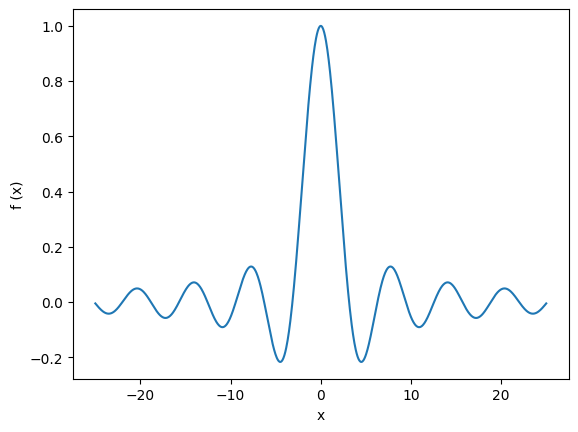
\includegraphics[width=0.50\textwidth]{sinx.png}
    \end{align*}

\begin{lstlisting}[language=Python, title=Fig. Python 1.2(a)]
## libraries
import numpy as np
from scipy.optimize import minimize

## obj func
def f(x):
    return np.sin(x) / x

## inits
init = [0, 5, 10, 15, 20, 25]

## algos
algo = ['BFGS', 'Powell', 'CG']

## solvers
for i in init:
    for j in algo:
        res = minimize(
            fun = f, 
            x0 = i , 
            method = j
        )
        
        ## results
        print(f'init = {i}, algo = {j}, x* = {np.round(res.fun, 4)}')
\end{lstlisting}

\begin{center}
    \begin{tabular}{lll}
        \textbf{Init. } & \textbf{Algo. } & \textbf{$x*$} \\
        0 & BFGS & - \\
        0 & Powell & -0.2172 \\
        0 & CG & -\\
        5 & BFGS & -0.2172 \\
        5 & Powell & -0.2172 \\
        5 & CG & -0.2172 \\
        10 & BFGS & -0.0913 \\
        10 & Powell & -0.0913 \\
        10 & CG & -0.0913 \\
        15 & BFGS & -0.0580 \\
        15 & Powell & -0.0580 \\
        15 & CG & -0.0580 \\
        20 & BFGS & -0.0580 \\
        20 & Powell & -0.0425 \\
        20 & CG & -0.0580 \\
        25 & BFGS & -0.0425 \\
        25 & Powell & -0.0425 \\
        25 & CG & -0.0425 \\
    \end{tabular}    
\end{center}\\~\\

The reason for the observed instability is that the non-convex objective function has many local minima. Different initialization points and algorithms may converge to different local minima or perhaps even fail to converge, as exhibited in the results. More advanced techniques may be necessary to obtain a higher quality solution.

\newpage
    \item Consider the optimization problem:
    \begin{equation}
        \begin{split}
            \text{min. } & x^2 \\
            \text{s.t. }
            & \sin(x) \leq 0
        \end{split}
    \end{equation}

\begin{lstlisting}[language=Python, title=Fig. Python 1.1(b)]
## libraries
import numpy as np
import matplotlib.pyplot as plt

## obj func
def f(x):
    return x**2

## const
def sin(x):
    return np.sin(x)

## plot
x = np.linspace(-25, 25, 1000)
y = sin(x)
plt.plot(x, y)
plt.xlabel('x')
plt.ylabel('sin(x)')
plt.axhline(
    y = 0, 
    color = 'grey', 
    linestyle = '--'
)
plt.show()
\end{lstlisting}
        \begin{align*}
            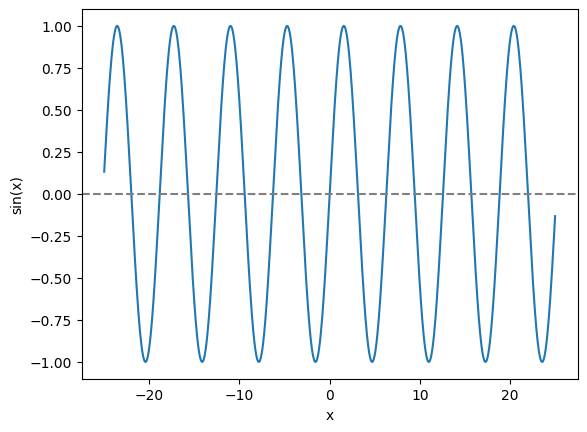
\includegraphics[width=0.50\textwidth]{sqrd.png}
        \end{align*}

\begin{lstlisting}[language=Python, title=Fig. Python 1.2(b)]
## libraries
import numpy as np
from scipy.optimize import minimize

## obj func
def f(x):
    return x**2

## const
def sin(x):
    return np.sin(x)

## inits
init = [1, 3, 6, 9, 12, 15]

## algos
algo = ['L-BFGS-B', 'TNC', 'CG']

## solvers
for i in init:
    for j in algo:
        res = minimize(
            fun = f, 
            x0 = i , 
            method = j,
            constraints = [sin(x = i)]
        )
        
        ## results
        print(f'init = {i}, algo = {j}, x* = {np.round(res.fun, 16)}')
\end{lstlisting}

    \begin{center}
        \begin{tabular}{lll}
            \textbf{Init.} & \textbf{Algo.} & \textbf{$x*$} \\
            1 & L-BFGS-B & 0.0 \\
            1 & TNC & 0.0 \\
            1 & CG & 1e-16 \\
            3 & L-BFGS-B & 0.0 \\
            3 & TNC & 0.0 \\
            3 & CG & 3e-16 \\
            6 & L-BFGS-B & 1.262e-13 \\
            6 & TNC & 0.0 \\
            6 & CG & 0.0 \\
            9 & L-BFGS-B & 0.0 \\
            9 & TNC & 0.0 \\
            9 & CG & 0.0 \\
            12 & L-BFGS-B & 4.54e-14 \\
            12 & TNC & 0.0 \\
            12 & CG & 1.48509e-11 \\
            15 & L-BFGS-B & 2.0195e-12 \\
            15 & TNC & 0.0 \\
            15 & CG & 9.1112e-12
        \end{tabular}
    \end{center}\\~\\

    Although the objective function, $x^2$, is convex, the feasible region of this problem is the set of all $x$ values that satisfy $\sin(x) \leq 0$, which is non-convex.  Therefore, the feasible region is non-convex, where standard optimization techniques might not converge to the same solution depending on the initialization point and algorithm.

    \end{enumerate}

\newpage
    \item The following program uses gradient search to minimize a function of two variables. It uses derivative-free bisection search to find the best step size at each iteration. For each iteration, the program prints out the iteration number, the current point, and the objective function value at the current point.
    
    The program to minimizes the function $f(x,y)=(x+y-2)^4+(x-2y+3)^2$. The gradient search algorithm starts from the point $(2,2)$ and continues to iterate while the point $(x_k, y_k)$ moves by a distance greater than the tolerance level of $0.001$ (i.e. $\sqrt{(x_k - x_{k-1})^2 + (y_k - y_{k-1})^2} > 0.001$).
    
    Bisection search utilizes a step size parameters are described below. The gradient search results clearly exhibit the final $x$ and $y$ coordinates that the algorithm converges to and the corresponding objective function value. The solution is near the global minimum.
    
    While running gradient descent, the bisection search algorithm determines the appropriate step size for each iteration of the gradient search algorithm. For bisection search, $a_k = 0, b_k = 10$, and $\epsilon_k = 0.1 \cdot (b_k - a_k)$ were specified. 
    
    Bisection search continues to iterate while the interval length $|b_k - a_k|$ is larger than the tolerance level $\theta = 0.001$. The step size is the midpoint of the interval that the bisection search stops. Bisection search prints the results for the first iteration of gradient search (used to find the first step size) at the initial starting point $(x, y) = (2, 2)$.
    
    To implement the gradient search algorithm with derivative-free bisection search, we define a function to evaluate the objective function and its gradient. Then we write a function to perform the bisection search and return the step size. Finally, we use these functions to implement the gradient search algorithm.\\

\begin{lstlisting}[language=Python, title=Fig. Python 2]
## library
import numpy as np

## obj func
def f(x, y):
    return (x + y - 2) ** 4 + (x - 2 * y + 3) ** 2

## grad vec
def df(x, y):
    dx = 4 * (x + y - 2) ** 3 + 2 * (x - 2 * y + 3)
    dy = 4 * (x + y - 2) ** 3 - 4 * (x - 2 * y + 3)
    return np.array([dx, dy])

## bisection search
def bisc_srch(f, x, y, dx, dy, ak=0, bk=10, epsk=1e-1, theta=1e-3):
    fk = f(x + dx * bk, y + dy * bk)
    fa = f(x + dx * ak, y + dy * ak)
    eps = epsk * (bk - ak)
    
    while bk - ak > theta:
        ck = (ak + bk) / 2
        fc = f(x + dx * ck, y + dy * ck)
        if fc < fa and fc < fk:
            return ck
        elif fa < fk:
            bk = ck
            fk = fc
        else:
            ak = ck
            fa = fc
    
    return (ak + bk) / 2

## gradient_descent
def grad_desc(f, df, x0, y0, alpha=0.1, theta=1e-3):

    x, y = x0, y0
    i = 0
    
    x_lst = list()
    y_lst = list()
    fx_lst = list()
    
    while True:
        fx = f(x, y)
        dfx, dfy = df(x, y)
        norm = np.sqrt(dfx ** 2 + dfy ** 2)
        
        if norm < theta:
            break
        
        step = bisc_srch(f, x, y, -dfx, -dfy)
        x -= alpha * step * dfx
        y -= alpha * step * dfy
        
        x_lst.append(x)
        y_lst.append(y)
        fx_lst.append(fx)
        
        i += 1

    ## results    
    print(f"Iteration 1: ({x0:.5f}, {y0:.4f}), f(x,y)={fx_lst[0]:.4f}")
    for j in range(1, i):
        print(f"Iteration {j+1}: ({x_lst[j]:.4f}, {y_lst[j]:.4f}), f(x,y)={fx_lst[j]:.4f}")
        
    return x, y, fx

## solver
x0, y0 = 2, 2
x, y, fx = grad_desc(f, df, x0, y0)
print(f"Optimiality: ({x:.4f}, {y:.4f}), f(x,y)={fx:.4f}")
\end{lstlisting}

    \begin{center}
        \begin{tabular}{lcl}
            Iter. & \textbf{($x, y$)} & \textbf{$f(x,y)$} \\
            1 & (2.0000, 2.0000) & 17.000 \\
            2 & (1.6805, 1.7548) & 10.727 \\
            3 & (1.5698, 1.6990) & 5.6150 \\
            4 & (1.4055, 1.6446) & 3.9647 \\
            5 & (1.2983, 1.6420) & 2.4622 \\
            6 & (1.1310, 1.6649) & 1.8103 \\
            7 & (1.0744, 1.6834) & 1.0431 \\
            8 & (1.0251, 1.7005) & 0.8305 \\
            9 & (0.9817, 1.7156) & 0.6667 \\
            10 & (0.9433, 1.7288) & 0.5395 \\
            . & . & . \\
            . & . & . \\
            . & . & . \\
            \textbf{99} & \textbf{(0.3710, 1.6855)} & \textbf{0.0000}
        \end{tabular}
    \end{center}\\~\\

    \item Consider the optimization problem:
        \begin{equation}
            \begin{split}
                \text{min. } & (x+y-2z)^2 +(2x-3y+z+1)^4 \\
                \text{s.t. }
                & x+z=3\\
                & 2y-x \leq 0.
            \end{split}
        \end{equation}

    \begin{enumerate}
        \item When formulated as an unconstrained optimization problem using the penalty function method, we have:
        \begin{equation}
            \operatorname*{min.}_{x\in\mathbb{R}} \quad (x+y-2z)^2 +(2x-3y+z+1)^4 + m_k (x+z-3)^2 + n_k(\max(0,2y-x))^2
        \end{equation}

        \item The following is a Python program to solve the constrained optimization problem using the penalty function method. It is initialized with $m = n = 10$, stopping tolerance $\theta = 0.1$, and magnifying parameter $\beta = 2$.\\

\begin{lstlisting}[language=Python, title=Fig. Python 3(b)]
## libraries
from scipy.optimize import minimize

## obj func
def f(x):
    y = x[1]
    z = x[2]
    return (x[0] + y - 2*z)**2 + (2*x[0] - 3*y + z + 1)**4

## const
def h(x):
    z = x[2]
    return x[0] + z - 3

def g(x):
    y = x[1]
    return x[0] - 2*y ## 'SLSQP' solves orig const, 2y-x <= 0

## penal
def pen(x, m, n):
    y = x[1]
    z = x[2]
    return f(x) + m*((h(x))**2) + n*(max(0, g(x)))**2

## init
m = n = 10
theta = 0.1
beta = 2
x0 = [0, 0, 0]

## toler
while True:

    ## const types
    st = (
        {'type': 'eq', 'fun': h},
        {'type': 'ineq', 'fun': g}
    )

    ## solver
    res = minimize(
        fun = pen, 
        x0 = x0,
        args = (m, n),
        constraints = st,
        method = 'SLSQP' ## converts x-2y >= 0 to 2y-x <= 0
    )
    x0 = res.x

    ## stopper
    if m*(h(x0))**2 + n*(max(0, g(x0)))**2 <= theta:
        break

    ## mag param
    else:
        m = beta*m
        n = beta*n

## results
print("(x*, y*, z*):", res.x)
print("min.:", res.fun)
\end{lstlisting}

    \begin{equation}
        \begin{split}
            x^* = 2.9942, \quad y^* &= 1.4971, \quad z^* = 0.0057\\
            min. &= 59.3118
        \end{split}
    \end{equation}\\
        
        \item The following two plots exhibit a convergence near zero when number of iterations increases: 1) the y-axis is the value of constraint term $x + z - 3$ in each iteration of solving the unconstrained problem, the x-axis is the number of iterations. 2) the y-axis is the value of constraint term $2y - x$ in each iteration of solving the unconstrained problem, the x-axis is the number of iterations.\\
        
\begin{lstlisting}[language=Python, title=Fig. Python 3(c)]
## libraries
from scipy.optimize import minimize
import matplotlib.pyplot as plt

## obj func
def f(x):
    y = x[1]
    z = x[2]
    return (x[0] + y - 2*z)**2 + (2*x[0] - 3*y + z + 1)**4

## const
def h(x):
    z = x[2]
    return x[0] + z - 3

def g(x):
    y = x[1]
    return x[0] - 2*y ## 'SLSQP' solves orig const, 2y-x <= 0

## penal
def pen(x, m, n):
    y = x[1]
    z = x[2]
    return f(x) + m*((h(x))**2) + n*(max(0, g(x)))**2

## init
m = n = 10
theta = 0.1
beta = 2
x0 = [0, 0, 0]

## const vals
i_num = list()
h_val = list()
g_val = list()

## toler
while True:

    ## solver
    res = minimize(
        fun = pen, 
        x0 = x0,
        args = (m, n),
        method = 'SLSQP' ## converts x-2y >= 0 to 2y-x <= 0
    )
    x0 = res.x

    ## const vals
    i_num.append(len(i_num) + 1)
    h_val.append(h(res.x))
    g_val.append(g(res.x))

    ## stopper
    if m*(h(x0))**2 + n*(max(0, g(x0)))**2 <= theta:
        break

    ## mag param
    else:
        m = beta*m
        n = beta*n

## plot const
plt.plot(i_num, h_val)
plt.xlabel("Iteration")
plt.ylabel("Constraint Value (x + z - 3)")
plt.show()

plt.plot(i_num, g_val)
plt.xlabel("Iteration")
plt.ylabel("Constraint Value (2y - x)")
plt.show()
\end{lstlisting}

        \begin{align*}
            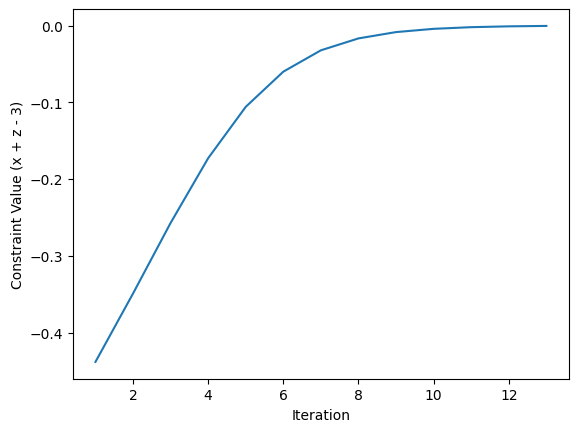
\includegraphics[width=0.50\textwidth]{cons1.png}
        \end{align*}
        \begin{align*}
            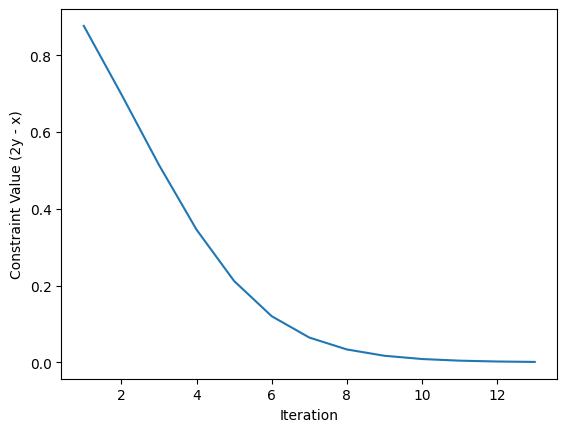
\includegraphics[width=0.50\textwidth]{cons2.png}
        \end{align*}

        The convergence of both constraint terms $x+z-3$ and $2y-z$ indicates that the penalty function method is effectively converting the constrained problem to an unconstrained problem with the desired constraints implicitly satisfied. Again, the two plots indeed exhibit a convergence near zero when the number of iterations increases.\\~\\

        \item Solving the original optimization problem by adding the constraints into the solver, we compare the solution to the one obtained by the penalty function method in part (b), where solution obtained using the penalty function method is the same as the constrained optimization method. This is because the penalty function method is effectively solving the same problem. In this case, the penalty function method in part (b), effectively converged to the same solution as the original problem below.\\

\begin{lstlisting}[language=Python, title=Fig. Python 3(d)]
## library
from scipy.optimize import minimize

## obj func
def f(x):
    y = x[1]
    z = x[2]
    return (x[0] + y - 2*z)**2 + (2*x[0] - 3*y + z + 1)**4

## const
def h(x):
    z = x[2]
    return x[0] + z - 3

def g(x):
    y = x[1]
    return x[0] - 2*y ## 'SLSQP' solves orig const, 2y-x <= 0

## init
x0 = [0, 0, 0]

## const types
st = (
    {'type': 'eq', 'fun': h},
    {'type': 'ineq', 'fun': g}
)

## solver
res = minimize(
    fun = f, 
    x0 = x0, 
    constraints = st, 
    method = 'SLSQP' ## converts x-2y >= 0 to 2y-x <= 0
)

## results
print("(x*, y*, z*):", res.x)
print("min.:", res.fun)
\end{lstlisting}

    \begin{equation}
        \begin{split}
            x^* = 2.9942, \quad y^* &= 1.4971, \quad z^* = 0.0057\\
            min. &= 59.3118
        \end{split}
    \end{equation}\\
        
    \end{enumerate}
%% end
\end{enumerate}
\end{document}
